\documentclass{article}

\usepackage{xspace}
\usepackage{amsmath}
\usepackage{graphicx}
\usepackage{natbib}
\usepackage{todo}
\usepackage[british]{babel}
\usepackage[left=1in,right=1in,top=1in,bottom=1in]{geometry}

\newcommand{\EE}{\ensuremath{E_\mathrm{E}}\xspace}
\newcommand{\EA}{\ensuremath{E_\mathrm{A}}\xspace}
\newcommand{\ED}{\ensuremath{E_\mathrm{D}}\xspace}
\newcommand{\Ed}{\ensuremath{E_\mathrm{d}}\xspace}
\newcommand{\p}{\vec{p}}
\newcommand{\q}{\vec{q}}

\newcommand{\dif}{\textup{d}}
\renewcommand{\vec}[1]{\mathbf{#1}}

\title{Formal definition of Retistruct algorithm}
\author{David C. Sterratt, Daniel L. Nedergaard and Ian D. Thompson}

\begin{document}
\maketitle
\thispagestyle{myheadings}

\section{Algorithm}
\label{fold-retina:sec:method}

This document gives a formal definition of the Retistruct definition,
with nomenclature that is mirrored in the Retistruct implementation.

\subsection{Triangulation of flattened retina}
\label{fold-sphere:sec:triang-flatt-retina}

% \begin{figure}[tp]
%   \centering
%   %\includegraphics{mesh}
%   \caption{Triangular mesh}
%   \label{fold-sphere:fig:mesh}
% \end{figure}

The edge of the flattened retina is described by a set of $N$ points:
$\mathcal{P} = \{\vec{p}_1,\dots,\vec{p}_N$\}. Connections between
points are represented by forwards and backwards pointers, which are
represented as vectors $\vec{g}^+$ and $\vec{g}^-$:
\begin{displaymath}
  g^+_i = \left\{
    \begin{array}{ll}
      i+1 & i < N \\
      1   & i = N
    \end{array}\right.
  \quad
  g^-_i = \left\{
    \begin{array}{ll}
      i-1 & i > 1 \\
      N   & i = 1
    \end{array}\right.
\end{displaymath}

A triangular mesh with the set of points $\mathcal{P}$ as its boundary
is created using the conforming Delaunay triangulation algorithm
provided by the Triangle package \citep{Shewchuk1996}. By summing the
areas of the triangles in this rough triangulation, the total area $A$
of the retina is computed. The retina is then triangulated again into
at least $n=200$ triangles, by using the conforming Delaunay
triangulation with the additional constraint that each triangle should
by no larger than $A/n$, and and with Ruppert's
\todo{Reference for Ruppert} method for ensuring the smallest angle of
any triangle is no less than $20^\circ$.

The triangulation comprises $M$ triangles and is described by an
$M\times3$ matrix $\mathbf{T}$, where each row contains the indices
of the points in the triangle in anticlockwise order.

The area $a_i$ of each triangle is computed:
\begin{displaymath}
  a_i = |0.5 (\vec{p}_{T_{i2}}-\vec{p}_{T_{i1}})\times
  (\vec{p}_{T_{i3}}-\vec{p}_{T_{i2}})|
\end{displaymath}

\begin{enumerate}
\item From the triangulation $\mathbf{T}$ the set $\mathcal{C}$ of pairs of
  indices representing line segments is constructed. 
\item For the morphing algorithm, it is essential that no line segment
  connects non-adjacent nodes in the rim $\mathcal{R}$. Such line
  segments may be created by the triangulation. To detect such line
  segments, each member of $\mathcal{C}$ is checked to see if it is a
  subset of $\mathcal{R}$ and that its ends are not adjacent, by
  using $g^+$ and $g^-$. For each line segment that is found, it is
  removed by
  \begin{itemize}
  \item removing the two triangles that it belongs to from the list
    $\mathbf{T}$
  \item Creating a new point at the centroid of the four vertices
    shared by these two triangles. This new point $i$ is added to the
    correspondences vector: $h_i=i$.
  \item Creating four new triangles, who all share the new point and
    the each of which has two vertices from the set of four
    triangles.
  \end{itemize}
\end{enumerate}

% The connection set is converted into $\mathbf{C}$, a symmetric,
% binary-valued matrix that defines if there is a connection between $i$
% and $j$.  

% The distances $L_{ij}$ are between grid points on the flattened retina
% are computed.

The connection set is converted into $\mathbf{C}$ a matrix with two
columns in which each row contains the indices of the connected
points $i$ and $j$. There is one row for each direction of the
connection. For example if point with index 3 and point with index 5
are connected, there would be two rows:
\begin{displaymath}
  \begin{array}{cc}
    3 & 5 \\
    5 & 3
  \end{array}
\end{displaymath}
There are $M$ rows in $\mathbf{C}$.

\subsection{Stitching algorithm}
\label{fold-sphere:sec:stitching-algorithm}

\begin{figure}[tp]
  \centering
  %\includegraphics{stitch}  
  \caption{Stitching. The solid line is the outline of the retina. The
    red circled-points are ones that were originally on the rim. The
    blue lines are the + tears and the purple lines are the - tears.
    Green lines indicate corresponding vertices at the end of tears.
    Yellow lines indicate corresponding points along the tears. }
  \label{fold-sphere:fig:stitch}
\end{figure}

Figure~\ref{fold-sphere:fig:stitch} shows a flattened
retina which has had the stitching algorithm applied to it. 

Cuts and tears marked up by an expert.  Each of the $M$ cuts or tears
$j$ is defined by a common apex at the point indexed by $A_j$, a
vertex in the forwards direction (indexed by $V^+_j$) and in the
backwards directions (indexed by $V^-_j$).  Pairs of vertices will
correspond to each other in the morphed retina, and this relationship
is indicated by a correspondence vectors $\vec{h}^+$ and $\vec{h}^-$:
\begin{displaymath}
  h^+_i =  \left\{
    \begin{array}{ll}
      i & \mbox{ if } i \not\in \{V^-_1,\dots, V^-_M\} \\
      V^+_j  & \mbox{ if } \exists j: i = V^-_j
    \end{array}\right.
  \quad
  h^-_i =  \left\{
    \begin{array}{ll}
      i & \mbox{ if } i \not\in \{V^+_1,\dots, V^+_M\} \\
      V^-_j  & \mbox{ if } \exists j: i = V^+_j
    \end{array}\right.
\end{displaymath}
At this stage, a correspondence vector $\vec{h}$ is initialised to be
the same as $\vec{h}^+$.

The set of points in each tear is determined using the function
$\mathrm{path}$:
\begin{displaymath}
  \mathrm{path}(i, j, \vec{g}, \vec{h})  = \left\{ 
  \begin{array}{ll}
    \{i\} & \mbox{ if } i = j \\
      \{i, \mathrm{path}(g_i, j, \vec{g}, \vec{h})\} & \mbox{ if } i \ne j, h_i=i \\
      \{i, \mathrm{path}(h_i, j, \vec{g}, \vec{h})\}    & \mbox{ if } i \ne j, h_i\ne i \\
    \end{array}\right.
\end{displaymath}
This allows us to write:
\begin{displaymath}
  \mathcal{T}^+_j  = \mathrm{path}(A_j, V_j^+, \vec{g}^+, \vec{h}^+) \quad 
  \mathcal{T}^-_j  = \mathrm{path}(A_j, V_j^-, \vec{g}^-, \vec{h}^-)
\end{displaymath}
It is useful to determine the set of points $\mathcal{R}$ on the rim
of the retina.
\begin{displaymath}
  \mathcal{R} = \{1,\dots,N\} 
  \setminus (\mathcal{T}^+_1 \setminus V^+_1) 
  \setminus (\mathcal{T}^-_1 \setminus V^-_1)  
  \dots 
  \setminus (\mathcal{T}^+_M \setminus V^+_M)
  \setminus (\mathcal{T}^-_M \setminus V^-_M)
\end{displaymath}

The function $\mathrm{pl}$ defines the path length from one point to another
point:
\begin{displaymath}
  \mathrm{pl}(i, j, \vec{g}, \vec{h}, \mathcal{P}) = \left\{ 
    \begin{array}{ll}
      0 & \mbox{ if } i = j \\
      |\vec{p}_i-\vec{p}_{g_i}| + \mathrm{pl}(g_i, j, \vec{g}, \vec{h}, \mathcal{P}) & \mbox{ if } i \ne j, h_i=i \\
      \mathrm{pl}(h_i, j, \vec{g}, \vec{h}, \mathcal{P})    & \mbox{ if } i \ne j, h_i\ne i \\
    \end{array}\right.
\end{displaymath}
For each tear, the length of each side of the tear is computed:
\begin{displaymath}
  S^+_j = \mathrm{pl}(A_j, V^+_j, \vec{g}^+, \vec{h}^+, \mathcal{P}) \quad 
  S^-_j = \mathrm{pl}(A_j, V^-_j, \vec{g}^-, \vec{h}^-, \mathcal{P})
\end{displaymath}
Then for each point $i$ on the $+$ side of the tear for which there is
no corresponding point $h_i^-$, a new, corresponding, point, with the
index $n=N+1$ is placed at the same fractional distance along the
corresponding $-$ tear. To do this, the distance of a point
$i\in{\mathcal{T}^+_j}\setminus A_j \setminus V^+_j$ along the + tear
is computed:
\begin{displaymath}
  s^+_{ji} = \mathrm{pl}(A_j, i, \vec{g}^+, \vec{h}^+, \mathcal{P}) \quad 
\end{displaymath}
The node $k$ in the corresponding tear is the node which has the node
with the highest fractional distance $s^-_{jk}=\mathrm{pl}(A_j, k,
\vec{g}^-, \vec{h}^-, \mathcal{P})$ along the $-$ tear which is still below
$s^+_{ji}$. The location of the new point is
\begin{displaymath}
  \vec{p}_n = (1-f)\vec{p}_k + f\vec{p}_{g^-_k}
\end{displaymath}
where
\begin{displaymath}
  f = \frac{s^+_{ji}S^-_j/S^+_j-s^-_{jk}}{s^-_{jg^-_k}-s^-_{jk}}
\end{displaymath}
The correspondences vector is updated so that $h_i = n$. The vector of
forward pointers is updated so that
\begin{displaymath}
  \begin{array}{ll}
    g^-_n = k     & g^+_n = g^+_k \\
    g^-_{g^+_k} = n & g^+_k = n 
  \end{array}
\end{displaymath}
If a correspondence $h^-_i$ exists for point $i$, then no new point is
made, but this point is set to correspond to the same point as $h^-_i$
corresponds to by setting $h_i = h_{h^-_i}$. 

A similar procedure is carried out for the $-$ tear.

After this procedure, it is possible that there may be chains of
correspondences where, for example, $i$ corresponds to $h_i$ and $h_i$
corresponds to a different point $h_{h_i}$. These three points are in
fact actually one, but to indicate this, both $h_i$ and $i$ should
point to $h_{h_i}$. It order to ensure this, the correspondence vector
is updated iteratively:
\begin{displaymath}
  h^{k+1}_i = h^k_{h^k_i}  
\end{displaymath}
until all $h^{k+1}_i = h^k_i$. The final $\vec{h}^{k+1}$ is referred
to as $\vec{h}$.

% The stitching algorithm uses this information to create
% correspondances between points on cuts and tears using an algorithm
% that


\subsection{Initial projection onto hemisphere}
\label{fold-sphere:sec:proj-onto-hemisph}

When the points are projected onto the hemisphere, the points which
the stitching algorithm has identified as corresponding with each
other are merged. This results in a new set of points, which is a
subset of the existing set of points created by the triangulation and
stitching operations. It is desirable to renumber this set of points
consecutively starting at 1. In order to do this, the following steps
are undertaken:
\begin{enumerate}
\item An ordered set $\mathcal{U}$ of the unique values of the range
  of $h$ is formed. $\mathcal{U}$ has $\tilde N$ elements. The mapping
  $u: \{1,\dots, \tilde N\} \rightarrow \mathcal{U}$ maps the new
  index to the old index. This this is a one-to-one mapping, $u$ is an
  invertable function.
\item A transformed set of points $\mathcal{\tilde P}$ is formed by
  setting $\tilde{\vec{p}}_i = \vec{p}_{u_i}$
\item A new mapping $\tilde h$ from the existing indices to a
  new set of unique indices is formed:
  \begin{displaymath}
    \tilde h_i = j:u_j = h_i \quad
    \tilde h(i) = u^{-1}(h(u(i)))
  \end{displaymath}
\item A transformed triangulation $\tilde{\mathbf{T}}$ is derived from
  $\mathbf{T}$, by setting $\tilde{T}_{ij} = \tilde h_{T_{ij}}$
\item A transformed rim set $\mathcal{\tilde R}$ is obtained by using
  $\tilde h_i$ to map every point $i$ in the the original rim set
  $\mathcal{R}$, formally: $\mathcal{\tilde R}: \{\tilde h_i
  \quad\forall i \in \mathcal{R}\} $
\end{enumerate}

It is also necessary to transform the indices used by the edge sets
and determine correspondences between edges which have been merged. A
mapping $H$ between connections (as opposed to points) is formed by
the following steps:
\begin{enumerate}
\item A transformed set of edges is formed by setting $C'_{ij} =
  \tilde h(C_{ij})$. A number of the rows of this matrix contain
  identical elements to each other. There is a mapping $H$ from each
  row of $\mathbf{C}$ to the corresponding row of $\mathbf{C'}$. This
  is analogous to the mapping $h$ for points. Mappings $\tilde{H}$ and
  $U$ are formed analogously to $\tilde{h}$ and $u$.
\item The final connection matrix $\tilde{\mathbf{C}}$ is formed using
  $U$ and $\mathbf{C}'$: $\tilde C_{ij} = C'_{u_iu_j}$. The number
  of rows in $\tilde{\mathbf{C}}$ is $\tilde M$.
\item The flattened lengths of most connections in stitched space
  remains the same as before. However connections that are matched to
  each other (along cuts) will have two original lengths, so we
  average these: $\tilde L_k = \frac{1}{|\mathcal{H}_k|}
  \sum_{i\in\mathcal{H}_k} L_i$ where $\mathcal{H}_k = i: k=H_k$.
\item In order to compute derivatives efficiently later on in the
  procedure, a we form a $\tilde N$ by $\tilde M$ matrix
  $\tilde{\mathbf{B}}$ which maps by setting $\tilde B_{\tilde
    C_{k1}k} = 1$ % and $\tilde B_{\tilde C_{k2}k} = 1$
  for all
  $k=1\dots \tilde M$.
\end{enumerate}

The total area $a_\mathrm{tot}$ of the retina is computed by summing the areas of
individual triangles:
\begin{displaymath}
  a_\mathrm{tot} = \sum_{i=1}^M a_i
\end{displaymath}
where $a_i = | a_i^\mathrm{sign}|$.  It is supposed that this grid is
to be projected onto a sphere with a radius appropriate for the area
$A$ of the flattened retina. The radius is
\begin{equation}
  \label{fold-sphere:eq:1}
  R = \sqrt{\frac{a_\mathrm{tot}}{2\pi\sin\phi_0+1}}
\end{equation}
where $\phi_0$ is the latitude at which the rim of the intact retina
would be expected. This function, and its derivative with respect to
$\phi_0$ is plotted in Figure~\ref{retistruct-algorithm:fig:R-phi}.

\begin{figure}
  \centering
  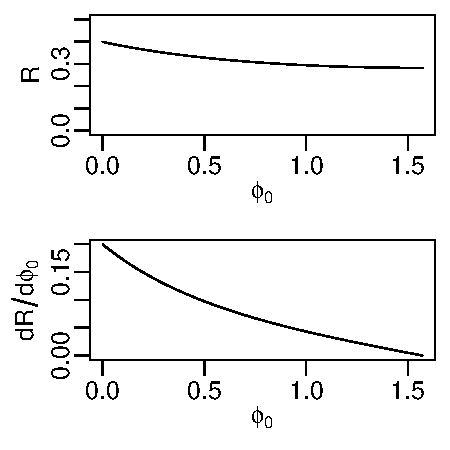
\includegraphics{R-phi}
  \caption{Upper plot: The radius $R$ as a function of $\phi_0$ for
    fixed area $a_\mathrm{tot}=1$. Lower plot: the derivative
    $\partial R/\partial \phi_0.$}
  \label{retistruct-algorithm:fig:R-phi}
\end{figure}

\subsection{Optimisation of the mapping}
\label{fold-sphere:sec:energy-function}

The aim now is to infer the latitude $\phi_i$ and longitude
$\lambda_i$ on the sphere to which each grid point $i$ on the
flattened retina is projected.  It is proposed to achieve this aim by
minimising an energy function which depends on two components, an
elastic component $E_\mathrm{E}$ and an area-preserving component
$E_\mathrm{A}$:
\begin{equation}
  \begin{split}
  E(\phi_1,\dots,\phi_N,\lambda_1,\dots,\lambda_N) = & \\
  E_\mathrm{E}(\phi_1,\dots,\phi_N,\lambda_1,\dots,\lambda_N) 
  & + \alpha E_\mathrm{A}(\phi_1,\dots,\phi_N,\lambda_1,\dots,\lambda_N) 
  \end{split}
\end{equation}
We will use an optimisation algorithm to find the set of values of
$\phi_i$ and $\lambda_i$ that minimise the energy.

The points on the rim are special cases. One of the points on the rim
is fixed to be in a known position on the eye (e.g.~the nasal or
dorsal position). We denote the index of this point $i_0$, and fix the
value of of its longitude $\lambda_{i_0}$. We can make two assumptions
about the latitude of the points on the rim:
\begin{enumerate}
\item Fixed rim angle: For the points on the rim (i.e.~$i \in
  \mathcal{\tilde R}$), $\phi_i$ is fixed to the value $\phi_0$
  supplied by the user, so we will not give it as a parameter to the
  optimisation algorithm.
\item Variable rim angle: For the points on the rim (i.e.~$i \in
  \mathcal{\tilde R}$), all $\phi_i$ have the same value $\phi_0$,
  which can vary, and should therefore be a parameter passed to the
  optimisation algorithm.
\end{enumerate}

To minimise $E$ we will use optimisation algorithms that require the
gradient of the energy with respect to $\phi_i$ and $\lambda_i$. In
the next sections we will compute these derivatives.

\subsubsection{Transformation between spherical coordinates and Cartesian
  coordinates on the sphere}
\label{retistruct-algorithm:sec:transf-betw-spher}

It turns out that we can simplify the calculations by:
\begin{enumerate}
\item Converting the spherical coordinates of each $(\phi_i, \lambda_i)$ to
   Cartesian coordinates $(x_i, y_i, z_i)$
 \item Calculating the partial derivatives of $\EE$ and $\EA$ with
   respect to $x_i$, $y_i$ and $z_i$
 \item Using the chain rule to compute the derivatives of $E$ with
   respect to $\phi_i$ and $\lambda_i$, and, if the rim angle varies,
   $\phi_0$:
\begin{equation}
  \begin{split} 
  \frac{\partial\EE}{\partial \phi_i} &  =
  \frac{\partial\EE}{\partial x_i}\frac{\partial x_i}{\partial
    \phi_i}
  +   \frac{\partial\EE}{\partial y_i}\frac{\partial y_i}{\partial
    \phi_i}
    +   \frac{\partial\EE}{\partial z_i}\frac{\partial z_i}{\partial
    \phi_i} \\
  \frac{\partial\EE}{\partial \lambda_i} &  =
  \frac{\partial\EE}{\partial x_i}\frac{\partial x_i}{\partial
    \lambda_i}
  +   \frac{\partial\EE}{\partial y_i}\frac{\partial y_i}{\partial
    \lambda_i}
    +   \frac{\partial\EE}{\partial z_i}\frac{\partial z_i}{\partial
      \lambda_i} \\
    \frac{\partial\EE}{\partial \phi_0} &  =
  \frac{\partial\EE}{\partial x_i}\frac{\partial x_i}{\partial
    \phi_0}
  +   \frac{\partial\EE}{\partial y_i}\frac{\partial y_i}{\partial
    \phi_0}
    +   \frac{\partial\EE}{\partial z_i}\frac{\partial z_i}{\partial
    \phi_0}
  \end{split}
\end{equation}
\end{enumerate}
In this section we will describe the coordinate transformation and
compute the derivatives of the Cartesian coordinates with respect to
the spherical coordinates.

To transform from spherical coordinates to Cartesian coordinates we us
the transformation:
\begin{equation}
  \vec{p}_i = 
  \label{retistruct-algorithm:eq:1}
  \left(
    \begin{array}{c}
    x_i\\ y_i\\ z_i
    \end{array}
  \right) =
  R\left(
    \begin{array}{c}
      \cos\phi_i\cos\lambda_i \\
      \cos\phi_i\sin\lambda_i\\
      \sin\phi_i 
    \end{array}\right)
\end{equation}
The derivatives of the Cartesian coordinates with respect to the
longitude and latitude are:
\begin{equation}
  \frac{\partial\vec{p}_i}{\partial\phi_i} = 
  \left(
    \begin{array}{c}
    \frac{\partial x_i}{\partial\phi_i}\\ \frac{\partial y_i}{\partial\phi_i}\\ \frac{\partial z_i}{\partial\phi_i}
    \end{array}
  \right) =
  R\left(
    \begin{array}{c}
      -\sin\phi_i\cos\lambda_i \\
      -\sin\phi_i\sin\lambda_i\\
      \cos\phi_i 
    \end{array}\right)
\end{equation}
\begin{equation}
  \frac{\partial\vec{p}_i}{\partial\lambda_i} = 
  \left(
    \begin{array}{c}
    \frac{\partial x_i}{\partial\lambda_i}\\ \frac{\partial y_i}{\partial\lambda_i}\\ \frac{\partial z_i}{\partial\lambda_i}
    \end{array}
  \right) =
  R\left(
    \begin{array}{c}
      -\cos\phi_i\sin\lambda_i \\
      \cos\phi_i\cos\lambda_i\\
      0
    \end{array}\right)
\end{equation}
If the rim angle is also allowed to vary, we also need the derivative
with respect to $\phi_0$, which we can obtain by using the product
rule:
\begin{equation}
  \frac{\partial\vec{p}_i}{\partial\phi_0} = 
  \left(
    \begin{array}{c}
      \frac{\partial x_i}{\partial\lambda_i}\\ \frac{\partial y_i}{\partial\phi_i}\\ \frac{\partial z_i}{\partial\phi_i}
    \end{array}
  \right) =
  \frac{\partial R}{\partial \phi_0}\left(
    \begin{array}{c}
      \cos\phi_i\cos\lambda_i \\
      \cos\phi_i\sin\lambda_i \\
      \sin\phi_i 
    \end{array}\right)
  +
  R\frac{\partial\phi_i}{\partial\phi_0}\left(
    \begin{array}{c}
      -\sin\phi_i\cos\lambda_i \\
      -\sin\phi_i\sin\lambda_i \\
      \cos\phi_i 
    \end{array}\right)
\end{equation}
Changing $\phi_0$ changes the radius $R$
(Equation~\ref{fold-sphere:eq:1}), which affects \emph{all} points
(the first term above). Changing $\phi_0$ also affects the latitudes
of the points on the rim, for which $\phi_i=\phi_0$. For these points
$\frac{\partial \phi_i}{\partial\phi_0}=1$, but for all other points
$\frac{\partial \phi_i}{\partial\phi_0}=0$.

\subsubsection{The elastic energy}
\label{fold-sphere:sec:elastic-force}

This component of the energy corresponds to the energy contained in
imaginary springs with the natural length of the distances in the
flattened retina, $\tilde L_k$:
% \begin{equation}
%   \label{fold-sphere:eq:5}
%   \EE  = \frac{1}{2} \sum_{i=1}^N \sum_{j=1}^N C_{ij} (l_{ij}-L_{ij})^2  
% \end{equation}
\begin{equation}
  \label{fold-sphere:eq:5}
  \EE  = \frac{1}{2} \sum_{k=1}^{\tilde M} \frac{(\tilde l_k- \tilde
    L_k)^2}{\tilde L_k}
\end{equation}
where $\tilde l_k$ is the distance of the $k$th edge between grid points on
the sphere and is given by:
\begin{equation}
  \label{fold-sphere:eq:2}
  \tilde l_k = 2R\arcsin\left(\frac{\sqrt{(x_i-x_j)^2 + (y_i-y_j)^2 + (z_i-z_j)^2}}{2R}\right)
\end{equation}
where $i=\tilde C_{k1}$ and $j=\tilde C_{k2}$.  Minimising this energy
function should lead to the distances between neighbouring points on
the sphere being similar to the corresponding distances on the
flattened retina.

% We aim to find the derivative of the elastic energy with respect to the
% Cartesian coordinates $\partial \EE/\partial x_i$, $\partial
% \EE/\partial y_i$ and $\partial \EE/\partial z_i$, and then use the
% chain rule to find the derivative of the elastic energy with respect
% to the latitude and longitude:
% \begin{equation}
%   \label{retistruct-algorithm:eq:6}
%   \begin{split} 
%   \frac{\partial\EE}{\partial \phi_i} &  =
%   \frac{\partial\EE}{\partial x_i}\frac{\partial x_i}{\partial
%     \phi_i}
%   +   \frac{\partial\EE}{\partial y_i}\frac{\partial y_i}{\partial
%     \phi_i}
%     +   \frac{\partial\EE}{\partial z_i}\frac{\partial z_i}{\partial
%     \phi_i} \\
%   \frac{\partial\EE}{\partial \lambda_i} &  =
%   \frac{\partial\EE}{\partial x_i}\frac{\partial x_i}{\partial
%     \lambda_i}
%   +   \frac{\partial\EE}{\partial y_i}\frac{\partial y_i}{\partial
%     \lambda_i}
%     +   \frac{\partial\EE}{\partial z_i}\frac{\partial z_i}{\partial
%     \lambda_i}
%   \end{split}
% \end{equation}

We compute $\frac{\partial\EE}{\partial x_i}$ using the chain rule:
\begin{equation}
  \label{retistruct-algorithm:eq:7}
  \begin{split}
    \frac{\partial\EE}{\partial x_i} & = \frac{\partial}{\partial x_i}
    \frac{1}{2} \sum_{k=1}^{\tilde M} \frac{(\tilde l_k- \tilde
      L_k)^2}{\tilde L_k} \\
    & = 
    \frac{1}{2} \sum_{k=1}^{\tilde M} \frac{\partial \tilde l_k}{\partial
      x_i} \frac{\partial }{\partial \tilde l_k}\frac{(\tilde l_k- \tilde
      L_k)^2}{\tilde L_k} \\
       & = 
       \sum_{k=1}^{\tilde M} \frac{\partial \tilde l_k}{\partial
      x_i} \frac{(\tilde l_k- \tilde
      L_k)}{\tilde L_k}
  \end{split}
\end{equation}

We now need to compute $\frac{\partial \tilde l_k}{\partial x_i}$.
There are two cases to consider:
\begin{enumerate}
\item If point $i$ is not one of the points at either end of link $k$
  (i.e.~if $i \ne C_{k1}$) then changing the value
  of $x_i$ has no effect on $\tilde l_k$ and so
  $\frac{\partial \tilde l_k}{\partial x_i}=0$
\item If point $i$ is one of the points at either end of link $k$
  (i.e.~if $i = C_{k1}$) then changing the value of $x_i$ affects
  $\tilde l_k$ and so $\frac{\partial \tilde l_k}{\partial x_i}$ can
  be non-zero. We will assume $i=C_{k1}$ and $j=C_{k2}$. Setting:
\begin{equation}
  \label{retistruct-algorithm:eq:2}
  v_k = \frac{\sqrt{(x_i-x_j)^2 + (y_i-y_j)^2 + (z_i-z_j)^2}}{2R}
\end{equation}
we can write the length \emph{over the surface of the sphere} as:
\begin{equation}
  \label{retistruct-algorithm:eq:8}
  \tilde l_k = 2R\arcsin v_k
\end{equation}
We then use the chain rule to differentiate $ \tilde l_k$ with respect
to each of the coordinates:
\begin{equation}
  \begin{split}
    \label{retistruct-algorithm:eq:4}
    \frac{\partial \tilde l_k}{\partial x_i} & = 2R \frac{\partial
      v}{\partial x_i}\frac{\dif}{\dif v_k}\arcsin v_k
    \quad \mbox{using the chain rule} \\
    & = 2R \frac{\partial
      v_k}{\partial x_i}\frac{1}{\sqrt{1-v_k^2}} \quad \mbox{derivative of
      $\arcsin v_k$} \\
    & = 2R \frac{1}{2R}\frac{2(x_i-x_j)}{2\sqrt{(x_i-x_j)^2 +
        (y_i-y_j)^2 + (z_i-z_j)^2}}\frac{1}{\sqrt{1-v_k^2}} \\
    & = \frac{(x_i-x_j)}{2Rv_k}\frac{1}{\sqrt{1-v_k^2}}
  \end{split}
\end{equation}
It turns out that using this derivative in an optimisation algorithm
leads to the algorithm becoming unstable, and that it is sufficient to
approximate the derivative by assuming that (a)~$v$ is close to zero,
which should be true because the the connections on the sphere only
subtend a small angle and (b)~$Rv_k\approx \tilde l_k \approx \tilde
L_k$, which holds because the the angle is small (so $v_k\approx
\arcsin v_k$ and the relaxed length should be similar to the original
length. Thus the derivative can be approximated to:
\begin{equation}
  \label{retistruct-algorithm:eq:10}
  \frac{\partial \tilde l_k}{\partial x_i} \approx
  \frac{(x_i-x_j)}{\tilde L_k}
\end{equation}
\end{enumerate}
Substituting Equation~\ref{retistruct-algorithm:eq:10} into
Equation~\ref{retistruct-algorithm:eq:7} for all links $k$ where point
$i$ is the first point in the connection pair leads to:
\begin{equation}
  \label{retistruct-algorithm:eq:9}
  \begin{split}
    \frac{\partial\EE}{\partial x_i} & = \sum_{k: C_{k1} = i}
      \frac{(x_i-x_{C_{k2}})}{\tilde L_k}
    \frac{(\tilde l_k- \tilde L_k)}{\tilde L_k}
  \end{split}
\end{equation}

We can apply the same principle to find the derivatives with respect
to $y_i$ and $z_i$ (here assuming case (2) above, that connection $k$
connects point $i$ to point $j$):
\begin{equation}
  \left(
    \begin{array}{c}
      \frac{\partial \tilde l_k}{\partial x_i} \\
      \frac{\partial \tilde l_k}{\partial y_i} \\
      \frac{\partial \tilde l_k}{\partial z_i}
    \end{array}
  \right) \approx
  \frac{1}{\tilde L_k}
  \left(
  \begin{array}{c}
    x_i-x_j \\
    y_i-y_j \\
    z_i-z_j
  \end{array}
  \right)
\end{equation}
We can write this in vector notation as:
\begin{equation}
  \label{retistruct-algorithm:eq:5}
  \frac{\partial \tilde l_k}{\partial \vec{p}_i} =   \frac{\vec{p}_i - \vec{p}_j}{\tilde L_k}
\end{equation}
We can also write Equation~(\ref{retistruct-algorithm:eq:9}) in vector notation:
\begin{equation}
  \label{retistruct-algorithm:eq:9}
  \begin{split}
    \frac{\partial\EE}{\partial \vec{p}_i} & = \sum_{k: C_{k1} = i}
      \frac{(\vec{p}_i-\vec{p}_{C_{k2}})}{\tilde L_k}
    \frac{(\tilde l_k- \tilde L_k)}{\tilde L_k}
  \end{split}
\end{equation}
The interpretation of this equation is that each component of the sum
is in the direction of the connection between $C_{k1}$ and $C_{k2}$
and that the energy increases when the connection is lengthened and
$\tilde l > \tilde L$, and that the energy decreases when the
connection is lengthened and $\tilde l < \tilde L$.

% In order to minimise the function efficiently, the derivatives with
% respect to $\phi_i$ and $\lambda_i$ are found:
% \begin{equation}
%   \label{fold-sphere:eq:3}
%   \begin{split}
%     \frac{\partial \EE}{\partial\phi_i} = 
%     \sum_j C_{ij} (l_{ij} - L_{ij})R
%     \frac{\sin\phi_i\cos\phi_j\cos(\lambda_i-\lambda_j) - \cos\phi_i\sin\phi_j}
%     {\sqrt{1-(\sin\phi_i\sin\phi_j +
%         \cos\phi_i\cos\phi_j\cos(\lambda_i-\lambda_j))^2}} \\
%     \frac{\partial \EE}{\partial\lambda_i} = 
%     \sum_j C_{ij} (l_{ij} - L_{ij})R
%     \frac{\cos\phi_i\cos\phi_j\sin(\lambda_i-\lambda_j)}
%     {\sqrt{1-(\sin\phi_i\sin\phi_j + \cos\phi_i\cos\phi_j\cos(\lambda_i-\lambda_j))^2}}
%   \end{split}
% \end{equation}
% A quasi-Newton-Raphson method is then used in R to achieve this
% optimisation, and the resulting grid on the sphere is plotted in 3D
% (Figure~\ref{fold-sphere:fig:test2}).

\subsubsection{The area-preserving energy}
\label{fold-sphere:sec:area-pres-energy}

\begin{figure}
  \centering
  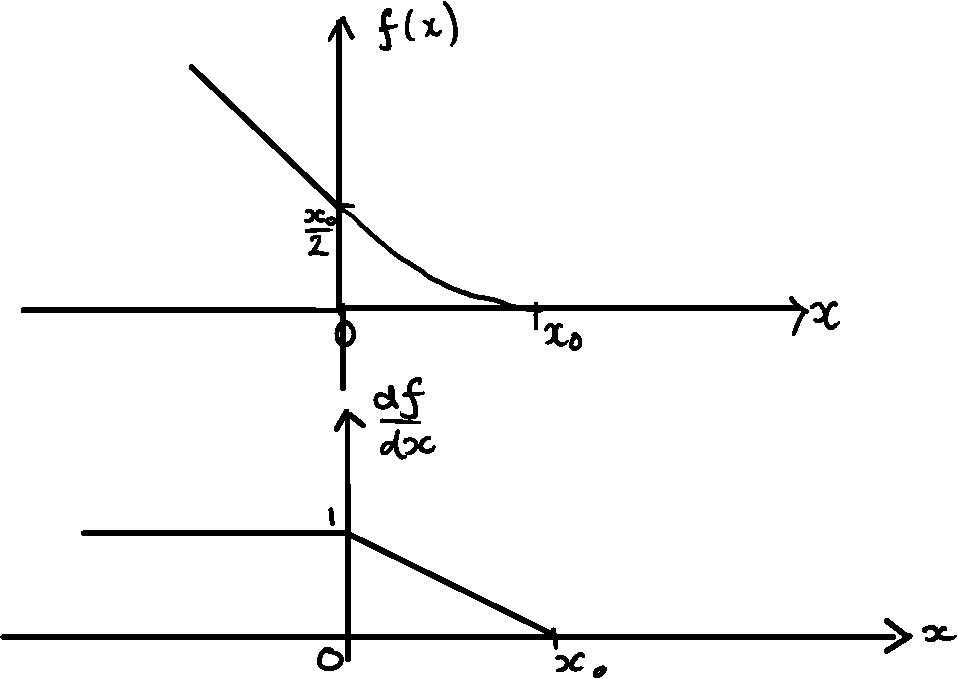
\includegraphics[width=0.5\linewidth]{area-f-crop.pdf}
  \caption{The function $f$ and its derivative with respect to $x$.}
  \label{retistruct-algorithm:fig:area-f}
\end{figure}

The area-preserving energy adds a penalty when the area of triangles
is very small or even negative:
\begin{equation}
 \EA = \sum_{t\in\mathcal{T}} f\left(\frac{a_t}{A_t}; x_0\right)
\end{equation}
where the function $f$ (Figure~\ref{retistruct-algorithm:fig:area-f}) is used to apply penalties mostly to
triangles with negative area, which are flipped:
\begin{equation}
  \label{retistruct-algorithm:eq:3}
  f(x) = \left\{
    \begin{array}{ll}
      -(x - x_0/2) & x < 0 \\
      \frac{1}{2x_0}(x - x_0)^2 & 0 < x <x_0 \\
      0 & x \ge x_0
    \end{array} \right.
\end{equation}
Here:
\begin{itemize}
\item $A_t$ and $a_t$ are signed areas of corresponding triangles
  $t\in\mathcal{T}$ in flattened and spherical retina
\item Signed area is positive for triangles in correct orientation,
  but negative for flipped triangles
\item Parameter $x_0$ should be small so that only triangles with
  negative or near-zero area ratios are penalised. Parameter $\alpha$
  scaled according to number of connections.
\end{itemize}

It is useful to write the coordinates of the points in terms of a unit
vector $\vec{e}_i$ and the radius:
\begin{equation}
  \label{retistruct-algorithm:eq:13}
  \vec{p}_i = R\vec{e}_i
\end{equation}
The signed area of a triangle $t$ formed by points $i=\tilde T_{t1}$,
$j=\tilde T_{t2}$ and $k=\tilde T_{t3}$ is:
\begin{equation}
  \label{retistruct-algorithm:eq:11}
  a_t = \frac{1}{2R} (\vec{p}_j\times \vec{p}_k)\cdot \vec{p}_i = \frac{R^2}{2} (\vec{e}_j\times \vec{e}_k)\cdot \vec{e}_i
\end{equation}
The derivative with respect to $\vec{p}_i$ is:
\begin{equation}
  \frac{\partial a_t}{\partial \vec{p}_i} = \frac{1}{2R} (\vec{p}_j\times \vec{p}_k)
\end{equation}
The derivative with respect to $R$ is 
\begin{equation}
  \label{retistruct-algorithm:eq:14}
  \frac{\partial a_t}{\partial R} =
  \frac{\partial}{\partial R} \frac{R^2}{2} (\vec{e}_j\times
  \vec{e}_k)\cdot \vec{e}_i
  = R (\vec{e}_j\times \vec{e}_k)\cdot \vec{e}_i = \frac{2a_t}{R}
\end{equation}

To calculate the derivatives with respect to the spherical coordinates
of the free points we use the chain rule:
\begin{equation}
  \label{retistruct-algorithm:eq:12}
  \begin{split}
  \frac{\partial \EA}{\partial \phi_i} = \sum_{t \in \mathcal{T}}
  \frac{\partial f}{\partial a_t}\frac{\partial a_t}{\partial
    \vec{p}_i}\frac{\partial \vec{p}_i}{\partial \phi_i} \\
  \frac{\partial \EA}{\partial \lambda_i} = \sum_{t \in \mathcal{T}}
  \frac{\partial f}{\partial a_t}\frac{\partial a_t}{\partial
    \vec{p}_i}\frac{\partial \vec{p}_i}{\partial \lambda_i} \\
  \end{split}
\end{equation}
If we are allowing the rim angle to vary we also need to calculate the
derivative with respect to $\phi_0$.
\begin{equation}
  \label{retistruct-algorithm:eq:12}
  \begin{split}
  \frac{\partial \EA}{\partial \phi_0} = \sum_{t \in \mathcal{T}}
  \frac{\partial f}{\partial a_t}
  \left(\frac{\partial a_t}{\partial \vec{p}_i}\frac{\partial
      \vec{p}_i}{\partial \phi_0} +
    \frac{\partial a_t}{\partial R}\frac{\partial
      R}{\partial \phi_0} 
  \right)\\
  \end{split}
\end{equation}
The one derivative we have not calculated already is $\frac{\partial
  R}{\partial \phi_0}$,which we calculate 
\begin{equation}
  \label{retistruct-algorithm:eq:15}
  \begin{split}
  \frac{\partial R}{\partial \phi_0} & = 2\pi\cos\phi_0
  \frac{a_\mathrm{tot}}{(2\pi\sin\phi_0 +1)^2}
  \frac{1}{2}\left(\frac{a_\mathrm{tot}}{2\pi\sin\phi_0+1}\right)^{-\frac{1}{2}}
  \\
  & =
  \frac{ \pi\cos\phi_0 a_\mathrm{tot}^{\frac{1}{2}}}{(2\pi\sin\phi_0 +1)^{\frac{3}{2}}}
    \end{split}
\end{equation}
where $\phi_0$ is the latitude at which the rim of the intact retina
would be expected.

\subsection{Mean location of points on sphere}
\label{fold-sphere:sec:mean-location-points}

The Karcher mean of a set of points on the sphere
\citep{Karcher1977,HeoSmall2006} is defined as the point
$(\overline{\phi}, \overline{\lambda})$ that has a minimal sum of
squared distances to the set of points $(\phi_i, \lambda_i)$:
%% See also BergWerm06
\begin{equation}
  \label{fold-sphere:eq:6}
  (\overline{\phi}, \overline{\lambda}) = \mbox{arg min}_{(\phi,
    \lambda)} \sum_{i=1}^N d^2(\phi, \lambda, \phi_i, \lambda_i)
\end{equation}
where (central angle)
\begin{equation}
  \label{fold-sphere:eq:7}
  d(\phi_i, \lambda_i, \phi_j, \lambda_j) = \cos\phi_i\cos\phi_j\cos(\lambda_i-\lambda_j) + \sin\phi_i\sin\phi_j  
\end{equation}
The generalised variance is
\begin{equation}
  \label{fold-sphere:eq:8}
  \sigma^2 = \frac{1}{N} \sum_{i=1}^N d^2(\overline{\phi}, \overline{\lambda}, \phi_i, \lambda_i)
\end{equation}

\bibliographystyle{apalike}
\bibliography{../paper/nmf_morph}


\end{document}

% LocalWords:  ij BP Raphson PDF myheadings RashEtal oppo shewchuk Ruppert's ji
%%% Local Variables: 
%%% TeX-PDF-mode: t
%%% End: 
% LocalWords:  jk th nmf Retistruct Ruppert iu Rv Karc riem HeoSmal
% LocalWords:  arg HeoSmall
